\section{Qualità di processo}

Per ottenere qualità, è necessario

\begin{itemize}
  \item Definire il processo, per poterlo facilmente controllare;
  \item Controllare il processo, per migliorarne efficienza ed efficacia;
  \item Usare buoni strumenti di valutazione.
\end{itemize}

\paragraph{Gestione della Qualità (QM)}
\label{par:gestione_della_qualit_}

La Gestione della Qualità assicura la consistenza di un'azienda, un prodotto o
un servizio. Ha quattro principali componenti:

\begin{itemize}
  \item Pianificazione della qualità;
  \item Controllo della qualità;
  \item Quality assurance;
  \item Miglioramento della qualità.
\end{itemize}

\paragraph{Sistema di Gestione della Qualità (SGQ)}
\label{par:sistema_di_gestione_della_qualit_}

Un Sistema di Gestione della Qualità (SGQ) è una \strong{collezione} di
\strong{processi} aziendali focalizzati al raggiungimento di obiettivi e
politiche di qualità per soddisfare i bisogni del cliente. Rappresenta la
struttura organizzativa, le politiche, le procedure, i processi e le risorse
necessarie a realizzare la Gestione della Qualità (Quality Management).

\subsection{ISO 9000}
\label{sub:iso_9000}

ISO 9000 è uno standard riguardante la gestione della qualità. Il suo obbiettivo
è di integrare un sistema di qualità in un'azienda, migliorando la produttività,
riducendo i costi non necessari e assicurando qualità di prodotto e di processo.

ISO 9000 rappresenta una famiglia di standard:

\begin{itemize}
  \item ISO 9000:2005: Fondamenti e glossario. Modelli di qualità neutri
    rispetto al dominio di applicazione;
  \item ISO 9001:2000: Sistema Gestione Qualità. ISO 9000 calata nei processi
    produttivi;
  \item ISO 90003:2004: Software engineering. Linee guida per l'applicazione di
    ISO 9001 al software.
\end{itemize}

\subsubsection{Documentazione del SGQ} % (fold)
\label{ssub:documentazione_del_sgq}

La normativa prevede della documentazione per la realizzazione del SGQ, tra cui
un Manuale della Qualità e un Piano della Qualità.

Il \strong{Manuale della Qualità} è il documento che definisce il sistema di
gestione della Qualità di un'organizzazione. Esprime una visione orizzontale (a
livello aziendale) e ad alto livello, integrandosi con le procedure aziendali e
fissando obiettivi di qualità e strategie attuative. Il Manuale di Qualità
esprime le \strong{politiche aziendali} rispetto alla qualità.

Il \strong{Piano della Qualità} è il documento che definisce gli elementi del
SGQ e le risorse che devono essere applicate in uno \strong{specifico caso}
(prodotto, processo, progetto). Rappresenta una visione strategica, verticale;
concretizza il Manuale della Qualità a livello di progetto, quindi sotto
specifici vincoli di tempo e risorse.

Il Piano di Qualità, nella pratica

\begin{itemize}
  \item Accerta la disponibilità di analisi dei requisiti, pianificazione e;
  risultati delle verifiche e delle prove;
  \item Accerta conformità ai modelli fissati dalle norme;
  \item Accerta tracciabilità da soluzioni e requisiti;
  \item Assicura la buona pianificazione delle attività (per uso di risorse).
\end{itemize}

\paragraph{Processi secondo ISO 9000}
\label{par:processi_secondo_iso_9000}

% Esatta copia delle slide. Da rivedere.

ISO 9000 soddivide i processi in quattro categorie:

\begin{itemize}
  \item Responsabilità della direzione;
  \item Gestione delle risorse;
  \item Realizzazione del prodotto;
  \item Misura, analisi e miglioramento.
\end{itemize}

\subsection{Strumenti di valutazione}
\label{sub:strumenti_di_valutazione}

\begin{itemize}
  \item Software Process Assessment \& Improvement (SPY): valutazione oggettiva
    dei processi di una organizzazione, per darne un giudizio di maturità e
    individuare azioni migliorative;
  \item (Capability Maturity Model Integration (CMMI): modello per la
    valutazioine uniforme dei fornitori;
  \item Software Process Improvement Capability dEtermination (SPICE): nato per
    armonizzare SPY con ISO/IEC 12207 e ISO 9001.
\end{itemize}

\subsubsection{Capability and Maturity Model Integration (CMMI)}
\label{ssub:capability_and_maturity_model_integration}

CMMI è un insieme strutturato di elementi che descrivono le caratteristiche di
processi efficaci. Costituisce una base concettuale su cui appoggiarsi per la
valutazione e il miglioramento dei processi, costruita su best-practice, e un
riferimento per valutare il miglioramento di un'azienda o confrontarne di
diverse.

\begin{itemize}
  \item \strong{Capability}: misura di quando un processo, considerato
    singolarmente, è adeguato in termini di efficienza ed efficacia;
  \item \strong{Maturity}: quanto il sistema dei processi dell'azienda è
    governato;
  \item \strong{Model}: insieme di requisiti di qualità per valutare il percorso
    di miglioramento;
  \item \strong{Integration}: architettura di integrazione delle diverse
    attività aziendali.
\end{itemize}

\begin{figure}[h!]
  \centering
  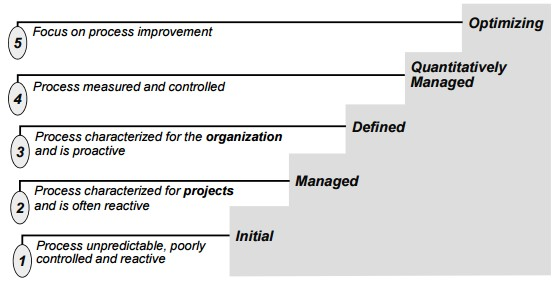
\includegraphics[scale=0.5]{imgs/cmmi_maturity_level}
  \caption{Livelli di maturità di CMMI}
\end{figure}

\subsubsection{ISO/IEC 15504 (SPICE)}
\label{ssub:spice}

ISO/IEC 15504, \frgnword{aka} SPICE, è un modello di riferimento per modelli di
maturità, utilizzando il quale si può valutare il livello generale di maturità
dell'azienda.

Il modello di riferimento definisce una \strong{dimensione di processo} e una
\strong{dimensione di capacità} (\frgnword{capability}).

La dimensione di processo divide i processi in cinque categorie:

\begin{itemize}
  \item Customer supplier;
  \item Engineering;
  \item Supporting;
  \item Management;
  \item Organization.
\end{itemize}

Per ogni processo, lo standard definisce un livello di capacità
(\frgnword {capability level}) sulla seguente scala:

\begin{enumerate}
  \item[0] Incomplete process;
  \item[1] Performed process;
  \item[2] Managed process;
  \item[3] Established process;
  \item[4] Predictable process;
  \item[5] Optimizing process.
\end{enumerate}

Lo standard specifica nove attributi di processo utilizzati per valutare la
capacità di processo, oltre che una metodologia di valutazione, che si compone
delle seguenti operazioni:

\begin{enumerate}
  \item Identificazione dei portatori d'interesse: i destinatari dei
    risultati e i responsabili dei processi valutati e delle attività di
    valutazione;
  \item Scelta tra valutazione e miglioramento: risultato a uso interno o
    esterno, valutazione formale o meno;
  \item Definizione della portata: processi inclusi nella valutazione,
    indicatori di valutazione.
\end{enumerate}
